After exposing all the necessary theory and context on \glspl{sn} and \glspl{osn}, we now present a more concrete image of the overall system. In Figure \ref{img:architectureprop} we present an abstract system architecture.

\begin{figure}[h!]
\begin{center}
  \hspace*{-0.3in}
  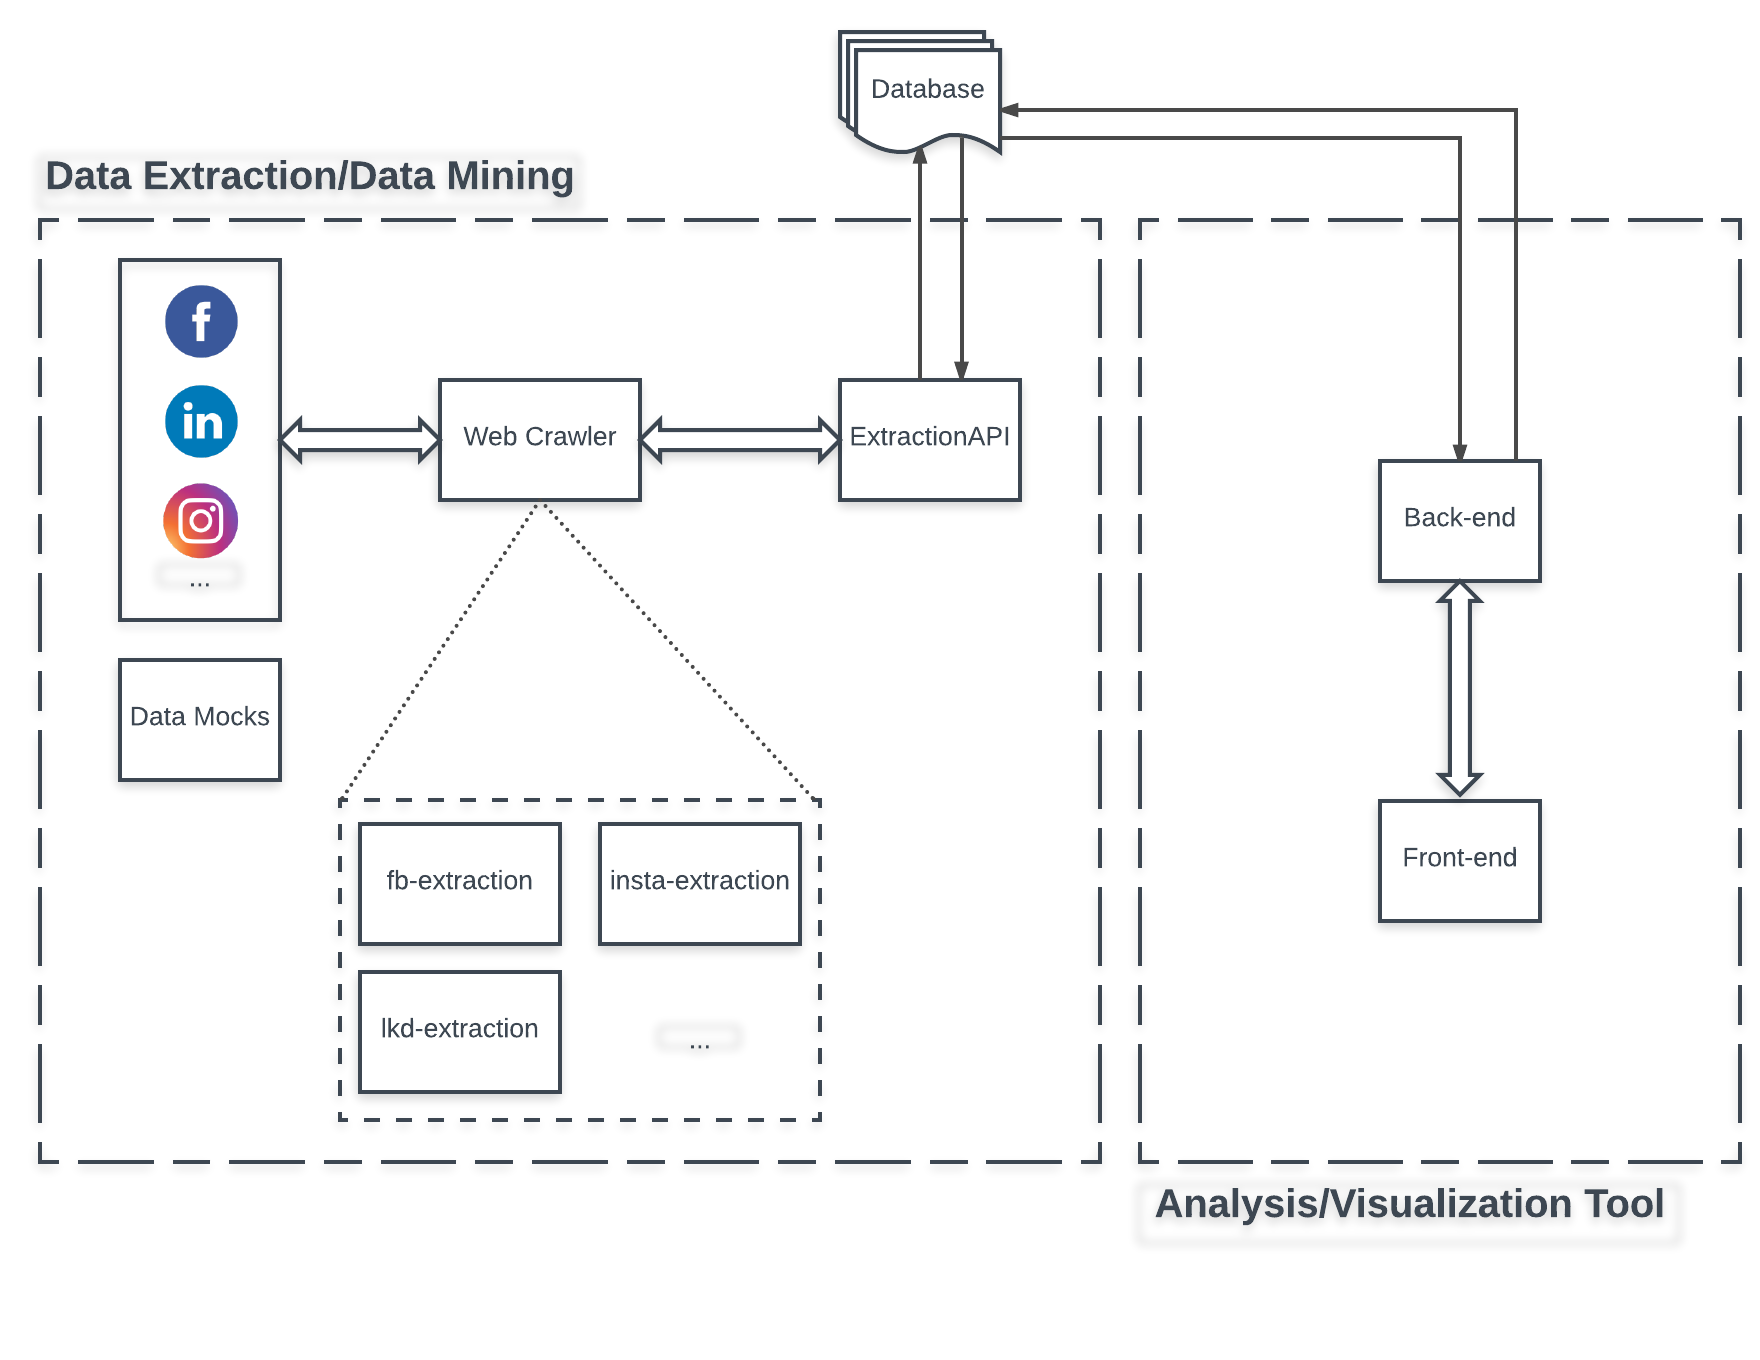
\includegraphics[width=1.1\textwidth]{img/architecture.png}
\end{center}
\caption{\label{img:architectureprop} System architecture proposal.}
\end{figure}

\section{General overview}
As the interaction of the software components may be clear from the diagram, the role of each module is not clear by simple
diagram observation, an underlying explanation of each component is needed in order to understand the system.\\
\indent We will follow a \textit{top down} approach for explaining the system architecture. First let us be clear about the two
main and distinct parts of the system:
\begin{itemize}
    \item \textbf{\textit{Information extraction and data mining}} - All the other components are built for extracting information
    from existent databases, or from \glspl{osn} (through the \textbf{Web Crawler}) and store information being information properly treated before stored;
    \item \textbf{\textit{Analysis and Application/Visualization}} - The tool that directly interacts with the end user is composed by a \textbf{Back-end} that fetches data from a database, runs calculations and algorithms on top of stored networks as the user requests by interacting with a \textbf{Front-end} that provides the visualization and interaction features.
\end{itemize}


\section{Detailed Components Description}
The components presented in Figure \ref{img:architectureprop} more detailed explanation, next we look more carefully into each on of the components.
\begin{itemize}
    \item \textbf{\textit{Data Mocks}} - This represents the strong hypothesis that we feed some data through data mocks, instead of crawling data from \gls{osn}. This data may be databases from projects that we already mentioned in this document  (\hyperref[sec:otherdatasources]{Section 3.3.6}), such as \cite{kunegis2013konect}. This data would be accessed through the \textbf{Extraction API}, or a new module could be constructed exclusively to feed this data to our database.
    \item \textbf{\textit{\acrfull{osn}}} - This are the object of study, the source of information that the systems will process and analyze;
    \item \textbf{\textit{Web Crawler}} - The \textbf{Web Crawler} consists in a set of modules for crawling each one of the \glspl{osn} (\textit{fb-extraction} and other modules).
    \item \textbf{\textit{ExtractionAPI}} - This module consists in a wrapper for extracting information from social networks, and allows extraction orchestration spreading extraction processes along multiple hosts, so that we can mitigate the slowness of web crawlers and extraction process in general;
    \item \textbf{\textit{Database}} - The database is where we store our data. It is not represented by the \textit{classical cilindro} because it resembles relational databases, and the possibility of using non relational databases such as document databases, grows strongly within the project, and the reason is the unstructured data that we will be storing into our database;
    \item \textbf{\textit{Back-end}} - Ideally this back-end component application will read the already normalized information from the database, run \glspl{sna} calculations and algorithms against the stored networks;
    \item \textbf{\textit{Front-end}} - The front-end will render the networks to the user, and will allow the user to interact with the network; these interactions will be defined in the requirements specifications.
\end{itemize}
